\chapter{Peridynamics Background}
\label{ch:PDBackground}

\section{Peridynamic States}
%
Introduced by Silling et al.\ in 2007~\cite{silling2007peridynamic}, peridynamic states are functions of the behavior of the continuum points surrounding each location.
As is appropriate for a theory based on force-carrying bonds, states often operate on vectors.
The most common states are scalar-states and vector-states which are scalar and vector valued, respectively.
As a matter of convention, scalar states are usually denoted by lowercase letters (e.g. $\sstate{a}{}{}$, $\sstate{b}{}{}$), while vector states are denoted by uppercase letters (e.g. $\vstate{A}{}{}$, $\vstate{B}{}{}$).
A state that operates on vectors and is itself vector valued naturally brings to mind a two-point tensor such as the deformation gradient;
unlike a second order tensor, which can only map vectors linearly to other vectors, vector-states can produce nonlinear, discontinuous, or even noninvertable mappings.  
This difference is illustrated in \cref{fig:VectorState}.
%
\begin{figure}[h]
  \centering
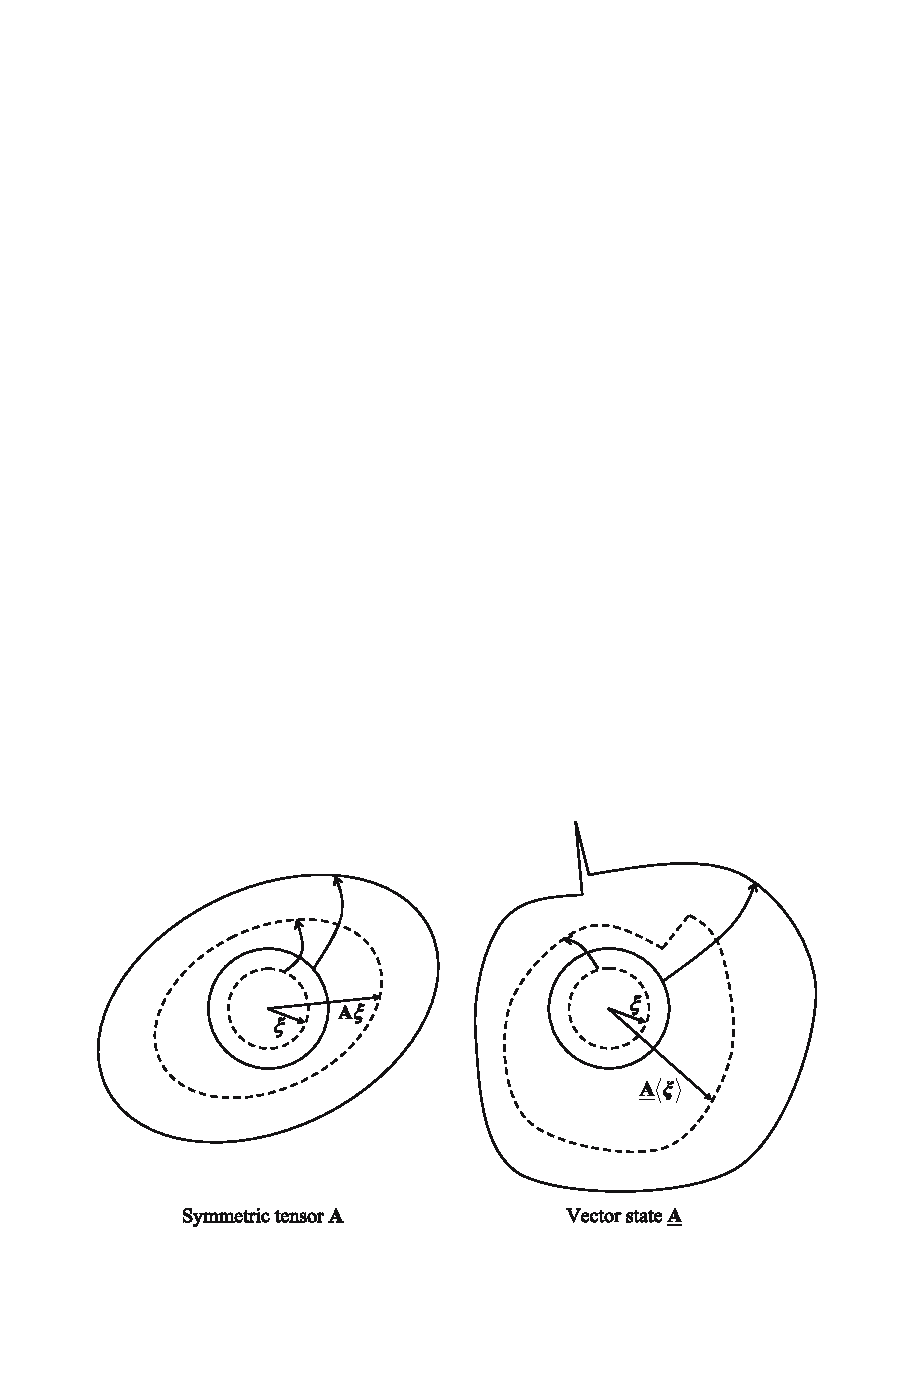
\includegraphics{VectorState}
\caption[Deformation tensor vs. deformation vector state]{The deformation tensor linearly maps spheres to ellipsoids, while a vector state can map spheres nonlinearly to complex and even discontinuous shapes \cite{silling2007peridynamic}}
\label{fig:VectorState}
\end{figure}
%

The mathematical properties of states and several related operators are defined in~\cite{silling2007peridynamic}.
Important properties of states are magnitude and direction, while important operations include the addition and composition of states, inner and tensor products, and the Fr\'{e}chet derivative of a function with respect to a state.
While some of these operations are intuitive, the nomenclature may not be.
Refer to \cref{table:StateOperations} for the notation of common state operations.
For a more rigorous definition and examples of the Fr\'echet derivative, see \cref{sec:frechet}.

\begin{table}
\centering
\caption{Common State Operation Nomenclature}
\begin{tabular}{l >{$\displaystyle}r<{$} >{$\displaystyle}l<{$}}
Operation & \textrm{Notation} & \textrm{Meaning} \\ \hline\hline
Addition & (\sstate{a}{}{} + \sstate{b}{}{})\langle\boldsymbol{\xi}\rangle & \sstate{a}{}{\boldsymbol{\xi}} + \sstate{b}{}{\boldsymbol{\xi}} \\ \hline
Multiplication & (\sstate{a}{}{}\sstate{b}{}{})\langle\boldsymbol{\xi}\rangle & \sstate{a}{}{\boldsymbol{\xi}}\sstate{b}{}{\boldsymbol{\xi}} \\  \hline
Scalar Product & (\vstate{A}{}{} \cdot \vstate{B}{}{})\langle\boldsymbol{\xi}\rangle & \vstate{A}{}{\boldsymbol{\xi}} \cdot \vstate{B}{}{\boldsymbol{\xi}} \\  \hline
Composition & (\vstate{A}{}{} \circ \vstate{B}{}{})\langle\boldsymbol{\xi}\rangle & \vstate{A}{}{ \vstate{B}{}{\boldsymbol{\xi}}}  \\ \hline \noalign{\smallskip}
\multirow{2}{*}{Dot Product} & \vstate{A}{}{} \bullet \vstate{B}{}{}& \int_\mathcal{H} \vstate{A}{}{\boldsymbol{\xi}} \cdot \vstate{B}{}{\boldsymbol{\xi}} \\ \noalign{\smallskip}
& \sstate{a}{}{} \bullet \sstate{b}{}{}&  \int_\mathcal{H} \sstate{a}{}{\boldsymbol{\xi}} \sstate{b}{}{\boldsymbol{\xi}} \\  \noalign{\smallskip} \hline \noalign{\smallskip}
Vector Norm & |\vstate{A}{}{}|\langle\boldsymbol{\xi}\rangle &  |\vstate{A}{}{}\langle\boldsymbol{\xi}\rangle|  \\\noalign{\smallskip} \hline\noalign{\smallskip}
State Norm & \|\vstate{A}{}{}\| & \sqrt{\vstate{A}{}{} \bullet \vstate{B}{}{}} \\ \noalign{\smallskip} \hline \noalign{\smallskip}
\multirow{2}{*}{Fr\'echet Derivative} & \nabla\mathit{f}(\vstate{A}{}{}) & \frac{\partial \mathit{f}}{\partial \vstate{A}{}{}} \\ \noalign{\smallskip}
& \Psi(\vstate{A}{}{},\vstate{B}{}{})_\vstate{A}{}{} & \frac{\partial \Psi}{\partial \vstate{A}{}{}} \\ \noalign{\smallskip} \hline\hline
\end{tabular}
\label{table:StateOperations}
\end{table}


\section{State-based Models}
Conservation of linear momentum in the \textit{state-based} peridynamic formulation results in the equation of motion
%
\begin{equation}
\label{eq:PDstateEoM}
\rho(\mathbf{x})\ddot{\mathbf{u}}(\mathbf{x}) = \int_\Omega (\vstate{T}{\mathbf{x}}{\mathbf{q}-\mathbf{x}}-\vstate{T}{\mathbf{q}}{\mathbf{x}-\mathbf{q}}) dV_\mathbf{q}  + \mathbf{b}(\mathbf{x})\, ,
\end{equation}
%
in which $\vstate{T}{\;}{\;}$ is a \textit{force vector-state} that maps the vector in angle brackets, $\langle \rangle$, originating at the point in square brackets, [ ], to a force vector acting on that point.
The deformed image of the vector $(\mathbf{q-x})$ is defined as the \textit{deformation vector-state}, usually denoted $\vstate{Y}{}{}$ and formulated 
%
\begin{equation}
%\label{eq:PDdeformation}
\vstate{Y}{\mathbf{x}}{\mathbf{q}-\mathbf{x}} = (\mathbf{q}-\mathbf{x}) + (\mathbf{u}(\mathbf{q})-\mathbf{u}(\mathbf{x})) 
\end{equation}
%
for a displacement field \(\mathbf{u}\). 
Just as stress and strain are work conjugate, so too are the force and deformation vector states for hyperelastic materials.

State-based models include surrounding material behavior illustrated in \cref{fig:pdDeformed} in the force function between each pair of continuum points. 
It is common for the formulation of the force state $\vstate{T}{}{}$ to be scaled by a weighting function, commonly represented by $\omega$, that makes explicit the region in which the force relationship between points is nonzero.
Perhaps the simplest and most common weight function is \cref{eq:WeightFunction}, representing a constant nonzero value for bonds shorter than the peridynamic horizon $\delta$.
%
\begin{equation}
\label{eq:WeightFunction}
\omega(\boldsymbol{\xi}) = 
\begin{cases}
1 & \text{if}\; |\boldsymbol{\xi}| \leq \delta\,, \\
0 & \text{if}\; |\boldsymbol{\xi}| > \delta\,.
\end{cases}
\end{equation}
%
Many evaluations of forces, energies, and other states at a given point are reduced from being integrals over the entire body to being integrals over that point's neighborhood $\mathcal{H}$.
This is particularly useful when trying to apply peridynamic models to real-world problems, especially when using computer models. 
%
\begin{figure}[h]
  \centering
\subinputfrom{\diagrampath}{PDbodyDeformed.eps_tex}
\caption{The body \protect\(\protect\Omega\protect\) deformed by the deformation state \protect\(\protect\vstate{Y}{}{}\protect\)}
\label{fig:pdDeformed}
\end{figure}
%
If the force state $\vstate{T}{}{}$ is always in the same direction as the deformation state $\vstate{Y}{}{}$, then the force exerted by a ``bond'' between points is in the same direction as the deformed bond, and the model is called \textit{ordinary}.  
Ordinary state-based models can reproduce linear elastic materials with arbitrary Poisson ratios by separating dilatory and deviatoric deformations and the energy corresponding to each.
%\begin{equation}
%\label{eq:wLPS}
%  \hat{W} ( \mathbf{\underline{Y}} ) = \frac{1}{2} \left( k - \frac{\alpha m}{9} \right) \vartheta^2+\frac{\alpha}{2} \int_{\mathcal{H}} \omega ( | \boldsymbol{\xi} | ) \underline{e}^2 \langle \boldsymbol{\xi} \rangle dV_{\boldsymbol{\xi}}
%\end{equation} 
They can also model a variety of elastic and inelastic behaviors.

There is no requirement that force states be in the same direction as their associated deformation states, and models in which they are not in the same direction are called \textit{nonordinary}.
Some additional care is needed to ensure that angular momentum is conserved in a \textit{nonordinary} state-based model, but they are still perfectly legitimate.
Silling et al.\ demonstrates the possibility of such models in \cite{silling2010peridynamic}, but very little work has touched on their use.  
Foster et al.\ \cite{foster2010viscoplasticity} and Warren et al.\ \cite{warren2009non} show that some correspondence models, which approximate the deformation gradient and use it to calculate bond forces, result in non-ordinary state-based constitutive models for finite deformations.
Bond-based, ordinary state-based, and nonordinary state-based models are illustrated in \cref{fig:PDmodelTypes}.
%
\begin{figure}[h]
  \centering
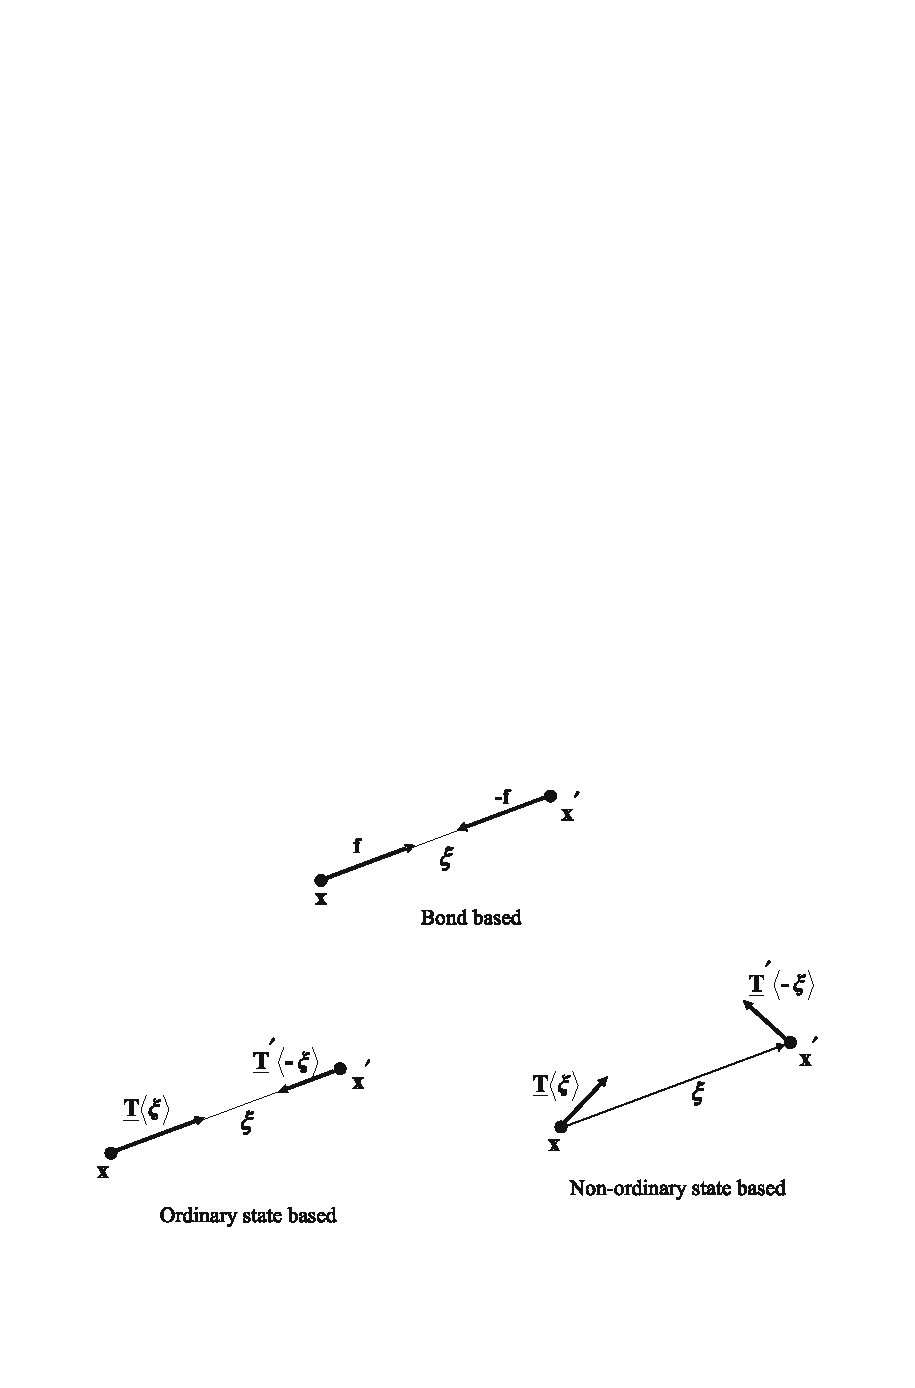
\includegraphics{PDmodelTypes}
\caption[Illustration of the three types of peridynamic models]{Illustration of the three types of peridynamic models, from specific to general \cite{silling2007peridynamic}}
\label{fig:PDmodelTypes}
\end{figure}

It should be clear that many of the concepts of classical continuum mechanics have direct equivalents in peridynamic modeling.
\Cref{table:PDconcepts} lays out some of the simplest parallels between classical and peridynamic formulations.

\begin{table}
\centering
\caption{Peridynamic Equivalents of Classical Concepts}
\begin{tabular}{l >{$\displaystyle}r<{$} >{$\displaystyle}l<{$}}
Concept & \textrm{Classical} & \textrm{Peridynamic} \\ \hline\hline
Kinematics & \mathbf{F} & \tvstate{Y}{}{} \\ \hline \noalign{\smallskip}
Linear Momentum & \nabla \cdot \boldsymbol{\sigma} & \int_\Omega (\vstate{T}{\mathbf{x}}{\mathbf{q}-\mathbf{x}}-\vstate{T}{\mathbf{q}}{\mathbf{x}-\mathbf{q}}) dV_\mathbf{q} \\    \noalign{\smallskip} \hline \noalign{\smallskip}
Angular Momentum &\boldsymbol{\sigma} = \boldsymbol{\sigma}^T  & \int_\Omega \vstate{Y}{\mathbf{x}}{\mathbf{q}-\mathbf{x}}\times\vstate{T}{\mathbf{x}}{\mathbf{q}-\mathbf{x}}dV_\mathbf{q} = 0\\   \noalign{\smallskip} \hline
Constitutive Law & \boldsymbol{\sigma} = \boldsymbol{\sigma}(\boldsymbol{\epsilon}) &\tvstate{T}{}{}=\tvstate{T}{}{}(\tvstate{Y}{}{}) \\  \hline
Stress Power  & \dot{\boldsymbol{\epsilon}} \boldsymbol{\sigma} &\tvstate{T}{}{}\bullet \tvstate{\dot{Y}}{}{} \\  \hline\hline
\end{tabular}
\label{table:PDconcepts}
\end{table}

\section{Bond-based peridynamics}
%
%If the force state \(\vstate{T}{\mathbf{x}}{\boldsymbol{\xi}} \) depends only on the deformation state \(\vstate{Y}{\mathbf{x}}{\boldsymbol{\xi}} \) \todo{This could be stated more simply by saying ``\ldots depends only on the deformed positions of the points at the end of a bond.''} of the same vector, then the model is called \textit{bond-based}.
If the force state \(\vstate{T}{\mathbf{x}}{\boldsymbol{\xi}} \) depends only on the deformed positions of the points at the end of the bond $\boldsymbol{\xi}$, then the model is called \textit{bond-based}.
In \textit{bond-based} peridynamic models, each pair of points is treated separately, without consideration of the behavior of other points. 
This makes bond-based models much simpler computationally than general state-based models, and reduces the equation of motion to
%
\begin{equation}
\label{eq:PDbondEoM}
\rho(\mathbf{x})\ddot{\mathbf{u}}(\mathbf{x}) = \int_\Omega \mathbi{f}(\mathbf{u}(\mathbf{q})-\mathbf{u}(\mathbf{x}),\mathbf{q}-\mathbf{x}) dV_\mathbf{q}  + \mathbf{b}(\mathbf{x})\, .
\end{equation}
%
By choosing an appropriate function $\mathbi{f}$, this model can reproduce the results of linear elasticity for solid materials with a Poisson ration \(\nu=\sfrac{1}{4}\) and 2-dimensional materials with a Poisson ration \(\nu=\sfrac{1}{3}\). 
It can also be used to investigate a range of nonlinear behaviors by changing the force function (examples in \cref{fig:BondForce}). 
To conserve momentum in a bond-based model, it is only necessary that $\mathbf{f}$ satisfy
%
\begin{equation}
\label{eq:PDbondF}
 \mathbi{f}(\mathbf{u}(\mathbf{q})-\mathbf{u}(\mathbf{x}),\mathbf{q}-\mathbf{x})=-\mathbi{f}(\mathbf{u}(\mathbf{x})-\mathbf{u}(\mathbf{q}),\mathbf{x}-\mathbf{q})\, ,
\end{equation}
%
i.e. the forces exerted at the opposite ends of the bond between $\mathbf{x}$ and $\mathbf{q}$ must be equal and opposite.
The first peridynamic models were all bond-based, and provide useful insight into many complex material failure phenomenon despite their limitations.
%
\begin{figure}[h]
  \centering
\subinputfrom{\diagrampath}{BondForce.eps_tex}
\caption{Bond-based models can describe a variety of material behaviors}
\label{fig:BondForce}
\end{figure}
%

\section{Important Peridynamic Models}
Though they cover only a small portion of the behaviors modeled with peridynamics, these few examples should serve to illustrate the form and analysis of peridynamic material models.
\subsection{Bond-based Elastic Solid}
The simplest peridynamic model treats each bond as a linear spring between two points.
In the bond-based formulation, there is no interaction between different bonds, so the force function is
%
\begin{equation}
\mathbi{f}(\mathbf{u}(\mathbf{q})-\mathbf{u}(\mathbf{x}),\mathbf{q}-\mathbf{x}) = \omega(|\mathbf{q}-\mathbf{x}|)\;c\;s \left[(\mathbf{q}+\mathbf{u}(\mathbf{q}))-(\mathbf{x}+\mathbf{u}(\mathbf{x}))\right]\, ,
\end{equation}
%
with weighting function $\omega$, spring constant $c$, and the stretch $s$ defined by
%
\begin{equation}
\label{eq:stretch}
s = |(\mathbf{q}+\mathbf{u}(\mathbf{q}))-(\mathbf{x}+\mathbf{u}(\mathbf{x}))| - |\mathbf{q}-\mathbf{x}|\, .
\end{equation}
%
For a deformation gradient $\mathbf{F}$ representing small uniform displacements, i.e. $\nabla \mathbf{u} << 1$, the stretch of bond $\boldsymbol{\xi}=\mathbf{q}-\mathbf{x}$ is
%
\begin{equation*}
s = |\mathbf{F}\boldsymbol{\xi}|-|\boldsymbol{\xi}| = \frac{\epsilon_{ij}\xi_i\xi_j}{|\boldsymbol{\xi}|}\, .
\end{equation*}
%
For reasons that will become clear in the discussion of the next model, we calibrate the spring constant $c$ following the approach of \cite{silling2007peridynamic}, by comparing the energy to that of a classical solid under purely deviatoric deformation, so that $\epsilon_{ij} = \epsilon_{ij}^d$.
The energy of this spring will be in units of energy per volume squared, so that integration over all the springs at a point gives energy per unit volume,
%
\begin{align}
\label{eq:deviatoricStrainEnergy}
w &= \frac{c\;s^2}{2}\, ,\notag \\
W &= \frac{c}{2}\int_\mathcal{H} \omega(|\xi|)\left( \frac{\epsilon_{ij}^d\xi_i\xi_j}{|\xi|} \right)\left( \frac{\epsilon_{kl}^d\xi_k\xi_l}{|\xi|} \right)\;dV_\xi\, ,\notag\\
&= \frac{c}{2}\epsilon_{ij}^d \epsilon_{kl}^d \int_\mathcal{H} \frac{\omega(|\xi|)}{|\xi|^2}\xi_i\xi_j\xi_k\xi_l \, .
\end{align}
%
Because $\omega$ depends only on $|\boldsymbol{\xi}|$, we can rewrite this integral in spherical coordinates as
%
\begin{equation}
W= \frac{c}{2}\epsilon_{ij}^d \epsilon_{kl}^d \int_0^\delta \frac{\omega(r)}{r^2}\int_0^{2\pi}\int_0^\pi (\xi_i\xi_j\xi_k\xi_l)\;r^2 \sin(\phi)\;d\phi\;d\theta\;dr\, .\notag
\end{equation}
%
Recognizing that $\xi_1 = r \sin\phi\cos\theta$, $\xi_2=r\sin\phi\sin\theta$, $\xi_3=r\cos\phi$, we can see that configurations of $[i,j,k,l]$ with an odd number of any index result in integrals with an odd number of one or more of $\cos\theta$, $\sin\theta$, $\cos\phi$, and therefor are equal to 0. 
For the remaining configurations,
%
\begin{equation}
\int_0^\delta \frac{\omega(r)}{r^2}\int_0^{2\pi}\int_0^\pi (r^4 \sin^4 \phi \cos^2\theta\sin^2\theta)\;r^2 \sin(\phi)\;d\phi\;d\theta\;dr =  \frac{4\pi}{15} \int_0^\delta \omega(r)r^4\;dr\, .\notag
\end{equation}
%
This leaves only configurations such as $[1,1,3,3]$, $[1,2,1,2]$ and $[3,2,2,3]$, which we can indicate by $(\delta_{ik}\delta_{jl}+\delta_{il}\delta_{jk}+\delta_{ij}\delta{kl})$ .
Additionally, any combination with $i=j$ or $k=l$ results in terms $\epsilon_{ii}^d$ or  $\epsilon_{kk}^d$.
Such terms sum to 0 in deviatoric deformation, leaving only $(\delta_{ik}\delta_{jl}+\delta_{il}\delta_{jk})$.
%
\begin{align}
W&= \frac{c}{2}\epsilon_{ij}^d \epsilon_{kl}^d \frac{4\pi}{15} \int_0^\delta \omega(r)r^4\;dr (\delta_{ik}\delta_{jl}+\delta_{il}\delta_{jk})\, ,\notag\\
&= c \;\epsilon_{ij}^d\epsilon_{ij}^d \frac{4\pi}{15} \int_0^\delta \omega(r)r^4\;dr\, , \notag\\
&= \frac{c\; \epsilon_{ij}^d\epsilon_{ij}^d }{15}m\, .\notag
\end{align}
%
To force the result to be independent of the horizon $\delta$, we normalize the expression by
%
\begin{equation}
\label{eq:weighted}
m=\int_\mathcal{H}\omega(|\boldsymbol{\xi}|)|\boldsymbol{\xi}|^2 = 4\pi \int_0^\delta \omega(r)\;r^4\;dr\, .
\end{equation}
%
By comparing to the classical strain energy density $\Omega = \mu\;\epsilon_{ij}^d\epsilon_{ij}^d$ for shear modulus $\mu$, we can determine the appropriate bond stiffness,
%
\begin{equation}
c = \frac{15\;\mu}{m}\, .\notag
\end{equation}
%
Applying a purely dilational deformation to the same model is far easier.
With dilation $\theta_{3D}$, the stretch of a bond in any direction is
%
\begin{equation}
s = \frac{\theta_{3D}}{3} r\, ,\notag
\end{equation}
%
and the corresponding energy is 
%
\begin{align}
W &= \frac{c}{2}\int_\mathcal{H} \omega(|\xi|)\frac{\theta^2_{3D}}{9} r^2 \;dV_\xi\, ,\notag\\
&=\frac{c\;\theta^2_{3D}}{18} \int_0^\delta \omega(r)\int_0^{2\pi}\int_0^\pi r^2\;r^2 \sin(\phi)\;d\phi\;d\theta\;dr\, , \notag\\
&= \frac{c\;\theta^2_{3D}}{18} m\, , \notag\\
&= \frac{15}{9}\mu\frac{\theta^2_{3D}}{2}\, .
\end{align}
%
This shows that the model based on bond-stretch has a bulk modulus that is \sfrac{15}{9} of its shear modulus, indicating a Poisson's ratio of \sfrac{1}{4}.

A nearly identical analysis can be performed on a simpler 2D version of the same model, departing after \cref{eq:deviatoricStrainEnergy}.
Applying a purely deviatoric in-plane shear to such a model, and comparing the resulting energy to that of a classical plate with thickness $t$ gives us
%
\begin{equation}
    c = \frac{8\;\mu\;t}{m_\textrm{2D}}\,,\qquad m_\textrm{2D} =\int_\mathcal{H_\textrm{2D}}\omega(|\boldsymbol{\xi}|)|\boldsymbol{\xi}|^2 dV_{\boldsymbol{\xi}}\, .  \notag
\end{equation}
%

Applying a planar dilation deformation to a 2D plate results in strain energy consistent with a Poisson's ratio of \sfrac{1}{3} rather than the value of \sfrac{1}{4} found for the 3D solid.

\subsection{State-based Elastic Solid}
The state-based linear isotropic peridynamic solid material model is both important and illustrative.
Developed in \cite{silling2007peridynamic}, it uses many of the important characteristics of peridynamic states to model a linearly-elastic material with any valid Poisson's ratio.
The extension state $\underline{e}$ is exactly the same as the stretch $s$ in \cref{eq:stretch}.
Classical material models dealing with metal plasticity often separate deformation into dilation and deviation components.
Similarly, the extension state can be decomposed into isotropic and deviatoric extension states. Using $m$ from \cref{eq:weighted} as above for normalization the dilation state is defined
%
\begin{equation}
    \theta_{3D} = \frac{3}{m} \int_\mathcal{H} \omega(\boldsymbol{\xi}) |\boldsymbol{\xi}| \underline{e} dV_{\boldsymbol{\xi}}\, .
\end{equation}
%
The isotropic and deviatoric extension states are defined in turn
%
\begin{equation}
\underline{e}^i = \frac{\theta_{3D} |\boldsymbol{\xi}|}{3},\qquad \underline{e}^d = \underline{e}-\underline{e}^i\, .
\end{equation}
%
If the energy associated with dilation is set to
%
\begin{equation}
W^i = \frac{k\;\theta^2_{3D}}{2}\, ,\notag
\end{equation}
%
then the corresponding force state is
%
\begin{equation}
\underline{t} = \frac{3k\theta_{3D}}{m}\omega(\boldsymbol{\xi})|\boldsymbol{\xi}|\, .\notag
\end{equation}
%
We saw in the analysis of the bond-based model the necessary bond stiffness to match the energy associated with purely deviatoric deformation.
The two can be combined for \cref{eq:lps}, a force state that clearly indicates the separate responses to dilation and deviatoric deformation:
%
\begin{equation}
\label{eq:lps}
\underline{t} = \frac{3k\theta_{3D}}{m}\omega(\boldsymbol{\xi})|\boldsymbol{\xi}| + \frac{15\;\mu}{m}\omega(\boldsymbol{\xi})\underline{e}^d\, .
\end{equation}
%
A quick examination shows that, in the case that the dilation $\theta_{3D}$ is not constant, the force at either end of a bond will not satisfy \cref{eq:PDbondF}.
Thus such a model is not possible in a bond-based framework without significant modification.
% \todo{If your looking to add a few pages the dissertation, you could include the recent work by Tupek on non-linear bond-strain models.  Just a thought.}

\subsection{Correspondence Models}
One way to create a peridynamic material model is to start from a material model in classical dynamics.
Classical models based on the deformation gradient have the advantage of decades of development and tens of thousands of hours of testing, and they enjoy widespread use in the continuum mechanics community.
Peridynamic \textit{correspondence} models use the relative positions of a points neighbors to determine $\bar{\mathbf{F}}(\vstate{Y}{}{})$, a nonlocal approximation of the deformation gradient $\mathbf{F}$.
%
\begin{equation}
\label{eq:PDapproxGradient}
\bar{\mathbf{F}}(\vstate{Y}{}{}) = \left[\int_\mathcal{H} \omega(|\boldsymbol{\xi}|)(\vstate{Y}{}{\boldsymbol{\xi}}\otimes \boldsymbol{\xi})\;dV_{\boldsymbol{\xi}} \right]\mathbf{K}^{-1}\, ,
\end{equation}
with the shape tensor $\mathbf{K}$ defined by
\begin{equation}
\mathbf{K} = \int_\mathcal{H}\omega(|\boldsymbol{\xi}|)(\boldsymbol{\xi} \otimes \boldsymbol{\xi})\;dV_{\boldsymbol{\xi}}\, . \notag
\end{equation}
%
When $\mathbf{F}$ is constant, $\bar{\mathbf{F}}(\vstate{Y}{}{})$ is exactly equal to $\mathbf{F}$.
If the classical model in question is hyperelastic with energy density $\Omega(\mathbf{F})$, it is a simple matter to force the peridynamic model to have identical energy by defining
\begin{equation}
W(\vstate{Y}{}{}) = \Omega(\bar{\mathbf{F}}(\vstate{Y}{}{}))\, ,
\end{equation}
and find the force vector state by taking the Fr\'echet derivative of $W$ with respect to $\vstate{Y}{}{}$.
Alternately, the classical continuum model can be applied to find the first Piola-Kirchhoff stress $\mathbf{P}$ associated with $\bar{\mathbf{F}}$:
\begin{equation}
\mathbf{P}=\frac{\partial\Omega(\bar{\mathbf{F}})}{\partial\bar{\mathbf{F}}}\, .
\end{equation}
The resulting force state is calculated from the stress according to
\begin{equation}
\vstate{T}{}{\boldsymbol{\xi}} = \omega(\boldsymbol{\xi})\mathbf{P}\mathbf{K}^{-1}\boldsymbol{\xi}\, .
\end{equation}
For homogenous deformations, the result is a peridynamic model that exactly reproduces the classical model without ever taking a derivative.
For problems with very inhomogenous (on the scale of the peridynamic horizon) deformations, the peridynamic model will exhibit scale effects not seen in the classical model, acting to smooth out the effect of short-scale deformations.
For discontinuous deformations, the classical model cannot be evaluated at all, but the peridynamic correspondence model will have no such problem.
It may be necessary however to revisit the choice of model or implement some damage condition. 

All three of these models are based on solid materials.
In such materials, the fundamental deformation mode is stretch or extension.
Consider instead a thin beam deflecting under transverse load; at the scale of the whole beam, the deflection behavior is the result of bending deformation.
To model the beam with a solid material model, it is necessary to use a much smaller scale - one in which the beam can be seen to stretch on one side and compress on the other.
Alternatively, in a model whose fundamental mode of deformation is bending, the same beam could be modeled at the same scale as its behavior.
